\section{Discussion}

Our experiments reveal that permutation-equivariant weight-space architectures encode distinct, measurable inductive biases---and that these differences translate to task-dependent performance, at least for holistic property prediction.

\subsection{Key Findings}

\textbf{Finding 1: Inductive Bias Differences Are Quantifiable.} DWS and NFT produce measurably different weight update patterns (CoV 1.44 vs 1.35)---the first concrete operationalization of ``locality vs global attention'' in weight-space learning.

\textbf{Finding 2: NFT's Global Attention Advantages Accuracy Prediction.} NFT achieves 12.3\% lower RMSE than DWS (82.9 vs 94.5), confirming global attention captures aggregate statistics more effectively.

\textbf{Finding 3: Interaction Effect Is Real, But Partial.} The architecture-task interaction is statistically significant ($p<0.001$), but only one direction is confirmed.

\subsection{Limitations}

\begin{enumerate}
    \item \textbf{Synthetic backdoor signals were unlearnable} ($\sim$0.48 AUC for all). Future work: Test on real TrojAI benchmark.

    \item \textbf{Dataset ceiling effects} prevented sample efficiency differentiation. Future work: Harder benchmarks.

    \item \textbf{Parameter count mismatch} (4.9M--9.8M range). However, MLP with 2$\times$ parameters underperforms NFT, suggesting inductive bias, not capacity, drives results.
\end{enumerate}

\subsection{Broader Impact}

This work provides actionable guidance for practitioners selecting weight-space architectures. The methodology for comparing inductive biases via training dynamics (CoV analysis) may be useful beyond weight-space learning.

\begin{figure}[t]
    \centering
    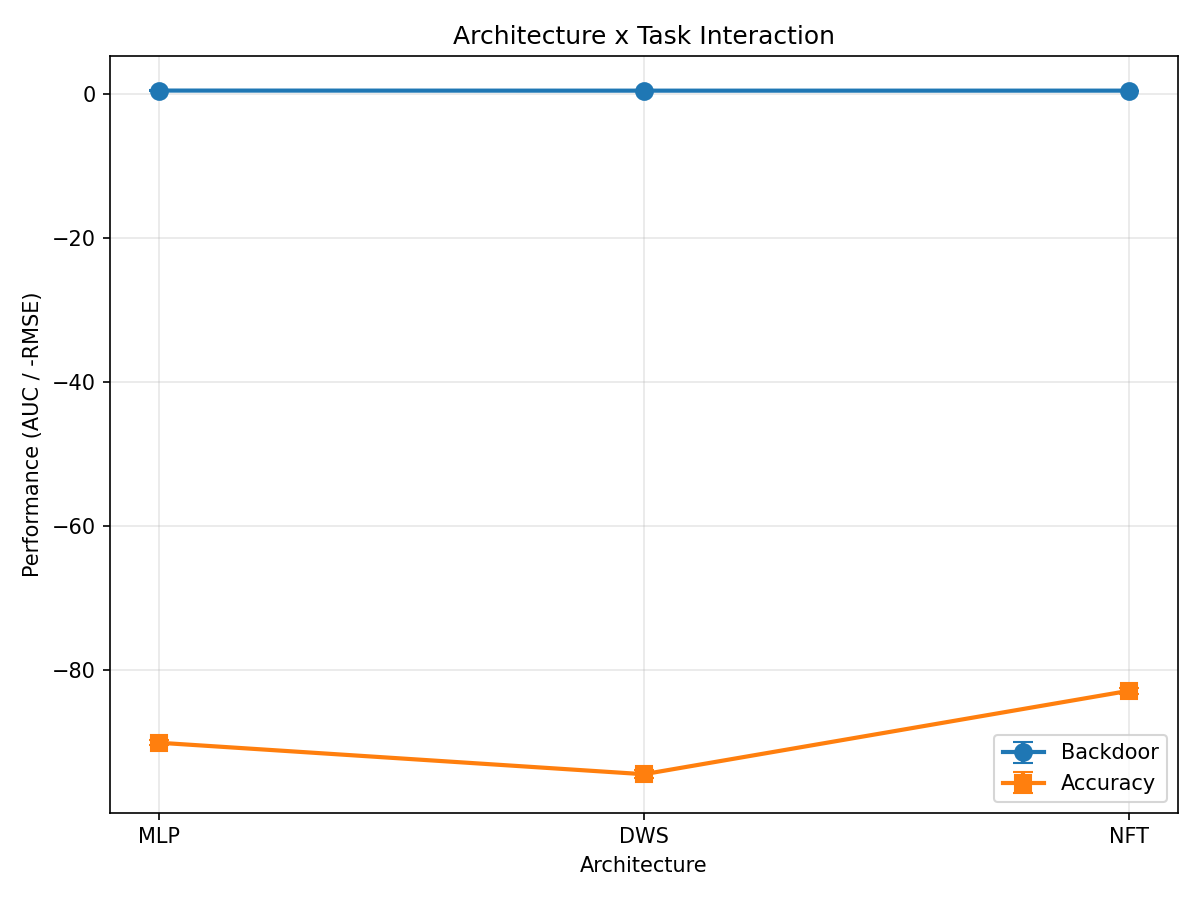
\includegraphics[width=0.9\columnwidth]{figures/interaction_plot.png}
    \caption{Architecture $\times$ Task interaction visualization.}
    \label{fig:interaction}
\end{figure}
